\documentclass{beamer}

\usepackage[utf8]{inputenc}
\usepackage[russian]{babel}
\usepackage{graphicx}

\usetheme{Warsaw}
\setbeamersize{text margin left=1em, text margin right=1em}
\usecolortheme{default}

\title[Генерация молекулярных строк с RNN]{ИССЛЕДОВАНИЕ МЕТОДОВ ПРЕДСТАВЛЕНИЯ И ГЕНЕРАЦИИ МОЛЕКУЛЯРНЫХ СТРОК С ИСПОЛЬЗОВАНИЕМ РЕКУРРЕНТНЫХ НЕЙРОННЫХ СЕТЕЙ}
\author{Кондратёнок Владимир Васильевич}
\institute[БГУ, ФПМИ]{
    БЕЛОРУССКИЙ ГОСУДАРСТВЕННЫЙ УНИВЕРСИТЕТ\\
    ФАКУЛЬТЕТ ПРИКЛАДНОЙ МАТЕМАТИКИ И ИНФОРМАТИКИ\\
    Кафедра биомедицинской информатики\\
    \textit{Научный руководитель: старший преподаватель, А.Д. Карпенко}
}
\date{Минск, 2025}

\begin{document}

\begin{frame}
    \titlepage
\end{frame}

\begin{frame}{Цели и задачи}
    \begin{block}{Цель работы}
        Комплексное исследование и сравнительный анализ современных методов представления и генерации молекулярных строк на основе нейронных сетей для задач целенаправленного дизайна молекул.
    \end{block}

    \begin{block}{Задачи}
        \begin{enumerate}
            \item Изучить теоретические основы представления молекулярных структур для задач машинного обучения, уделив особое внимание нотации SMILES.
            \item Рассмотреть базовые архитектуры генеративных моделей (RNN, VAE) и их раннее применение.
            \item Провести детальный анализ современных подходов к целевой генерации, включая оптимизацию в латентном пространстве и обучение с подкреплением (RL).
            \item Исследовать проблемы стандартизации оценки моделей и определить перспективные направления развития.
        \end{enumerate}
    \end{block}
\end{frame}

\begin{frame}[shrink=15]{Представление молекул: SMILES}
    \begin{columns}[T]
        \begin{column}{0.5\textwidth}
            \begin{block}{SMILES (Simplified Molecular-Input Line-Entry System)}
                Формат, представляющий молекулу в виде строки символов ASCII. Позволил применить методы обработки естественного языка (NLP) к задачам медицинской химии.
            \end{block}
            \begin{block}{Основные правила кодирования}
                \begin{itemize}
                    \item \textbf{Атомы:} Стандартные символы (C, N, O). Строчные буквы для ароматических систем.
                    \item \textbf{Связи:} Одинарные по умолчанию, `=` для двойных, `\#` для тройных.
                    \item \textbf{Ветвления:} В круглых скобках `()`.
                    \item \textbf{Циклы:} Разрыв связи в цикле, атомы помечаются одинаковыми цифрами.
                \end{itemize}
            \end{block}
        \end{column}
        \begin{column}{0.5\textwidth}
            \centering
            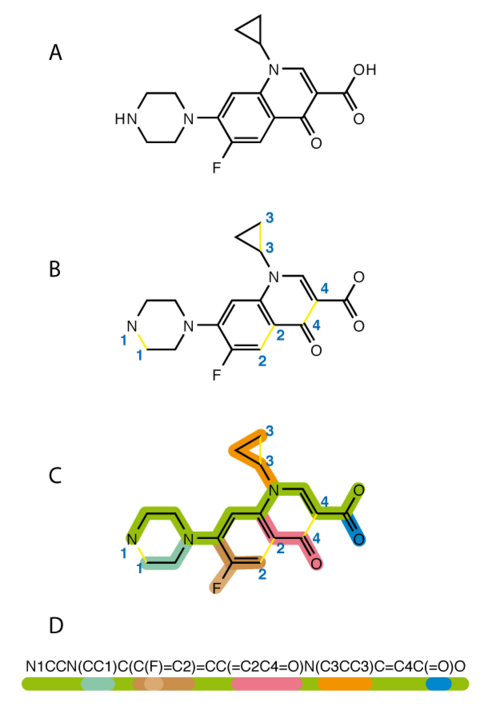
\includegraphics[width=0.85\textwidth]{images/smiles.png}
            \tiny
            Ципрофлоксацин
        \end{column}
    \end{columns}
\end{frame}

\begin{frame}{Альтернативные представления молекул}
    \begin{block}{Проблемы SMILES}
        \begin{itemize}
            \item \textbf{Неканоничность:} Одна молекула может быть представлена множеством строк (например, CCO и OCC для этанола).
            \item \textbf{Синтаксические ошибки:} Модели часто генерируют невалидные строки (например, с непарными скобками).
        \end{itemize}
    \end{block}

    \begin{block}{Альтернативы}
        \begin{itemize}
            \item \textbf{InChI (International Chemical Identifier):} Гарантирует абсолютно уникальную, каноническую строку для любой структуры.
            \item \textbf{Молекулярные графы:} Наиболее естественное представление (атомы -- узлы, связи -- ребра). Исключает синтаксически невалидные структуры.
            \item \textbf{SELFIES (Self-referencing embedded strings) и fragSMILES:} Гарантирует 100\% синтаксическую валидность генерируемых строк.
        \end{itemize}
    \end{block}
\end{frame}

\begin{frame}{Современные подходы к целевой генерации}
    Две основные философии:
    \begin{enumerate}
        \item \textbf{Оптимизация в латентном пространстве (VAE/Гетероэнкодеры)}
        \begin{itemize}
            \item Непрямой контроль.
            \item Задача: построить качественное, непрерывное представление химического пространства.
            \item Генерация и оптимизация являются вторичными задачами, выполняемыми внутри этого пространства.
        \end{itemize}
        \vspace{0.5cm}
        \item \textbf{Прямая оптимизация политики (Обучение с подкреплением, RL)}
        \begin{itemize}
            \item Прямой контроль.
            \item Задача: напрямую максимизировать заданную функцию вознаграждения (например, аффинность связывания).
            \item Модель обучается генерировать образцы, которые получают высокий балл.
        \end{itemize}
    \end{enumerate}
    \centering
\end{frame}

\begin{frame}[shrink=20]{Подход 1: Гетероэнкодер}
    \begin{block}{Проблема стандартного автоэнкодера}
    Разные SMILES-представления одной и той же молекулы отображаются в удаленные точки латентного пространства, делая его «зашумленным» и непригодным для навигации.
    \end{block}
    
    \begin{block}{Решение: Гетероэнкодер}
    Решает задачу «перевода» между различными, но семантически эквивалентными представлениями. Например, из канонической SMILES-строки в одну из множества случайных. Это заставляет модель изучать инвариантное, химически релевантное представление молекулы.
    \end{block}
    
    \centering
    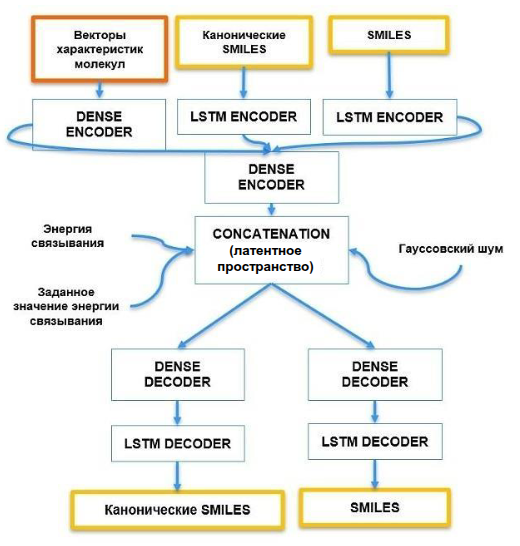
\includegraphics[height=6cm]{images/heteroencoder.png}
\end{frame}


\begin{frame}[shrink=20]{Подход 2: Reinforcement Learning (RL)}
    \begin{block}{Основная идея}
        Прямое обучение генеративной модели (агента) максимизировать целевую функцию (вознаграждение) путем итеративного взаимодействия со «средой».
    \end{block}
    
    \begin{block}{Ключевые компоненты (фреймворк REINVENT)}
        \begin{itemize}
            \item \textbf{Состояние}: Текущая молекула.
            \item \textbf{Агент:} Генеративная модель (RNN), которая генерирует молекулы в виде SMILES-строк.
            \item \textbf{Действие}: Химический фрагмент для присоединения.
            \item \textbf{Среда:} Программный модуль, вычисляющий скалярную оценку (вознаграждение) для молекулы (QSAR, докинг).
            \item \textbf{Вознаграждение:} Целевая функция, которую агент стремится максимизировать.
        \end{itemize}
    \end{block}
    
    \centering
    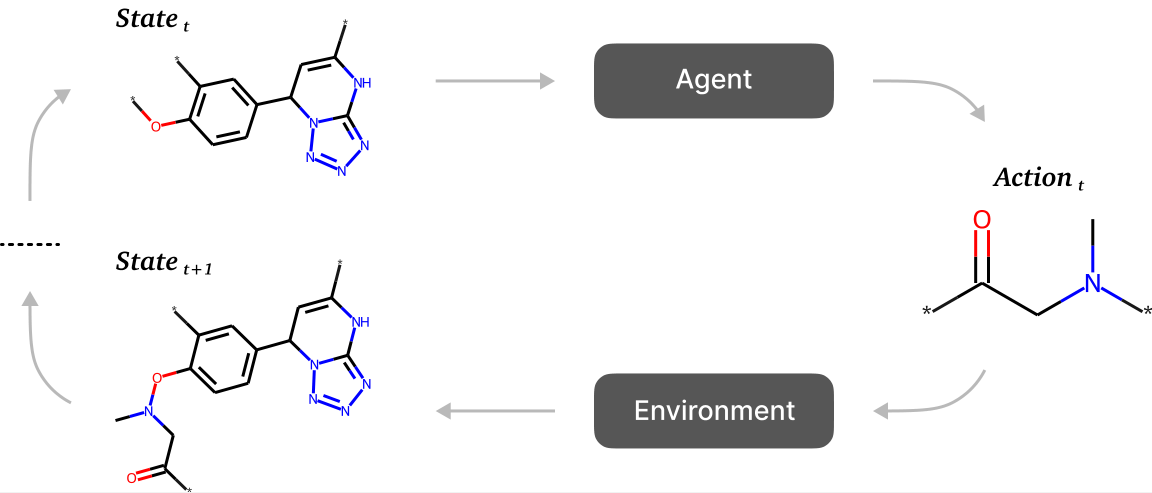
\includegraphics[height=3.5cm]{images/RL.png}
\end{frame}


\begin{frame}{Сравнительный анализ подходов}
    \begin{table}
    \centering
    \resizebox{\textwidth}{!}{
    \begin{tabular}{|l|p{4.5cm}|p{4.5cm}|}
        \hline
        \textbf{Критерий} & \textbf{Оптимизация в латентном пространстве} & \textbf{Прямая оптимизация} \\
        \hline
        \textbf{Разнообразие} & Высокое. Модель аппроксимирует распределение данных. & Потенциально низкое. Склонность к эксплуатации найденных решений. \\
        \hline
        \textbf{Требования к данным} & Требуется крупный и разнообразный набор данных для обучения. & Используется предобученная модель. Не требуется специфический набор данных для оптимизации. \\
        \hline
        \textbf{Гибкость} & Низкая. Интеграция нового свойства требует переобучения. & Высокая. Новые свойства легко добавляются в функцию вознаграждения. \\
        \hline
        \textbf{Интерпретируемость} & Относительно высокая. Структура латентного пространства допускает визуализацию. & Низкая. Процесс принятия решений трудно интерпретируем. \\
        \hline
    \end{tabular}
    }
    \end{table}
\end{frame}

\begin{frame}{Стандартизация оценки: бенчмарк MOSES}
    \begin{block}{Проблема}
        Отсутствие единого стандарта для сравнения генеративных моделей. Исследователи использовали разные наборы данных и метрики, что делало невозможным объективное сравнение.
    \end{block}

    \begin{block}{MOSES (Molecular Sets)}
        Бенчмарк, сосредоточенный на задаче обучения распределению.
        \begin{itemize}
            \item Предоставил большой, тщательно отфильтрованный набор данных.
            \item Ввел комплексный набор метрик для оценки (валидность, новизна, уникальность).
            \item Предложил специальный тестовый набор на основе \textbf{скаффолдов}, который позволяет оценивать способность моделей к генерализации и созданию молекул с новыми химическими каркасами.
        \end{itemize}
    \end{block}
\end{frame}

\begin{frame}{Перспективы развития}
    \begin{block}{Направление №1: От RNN к Трансформерам и большим языковым моделям}
    Архитектура Трансформер, благодаря механизму внимания, способна улавливать дальние зависимости в последовательностях, что делает ее более мощным инструментом для моделирования сложных SMILES-строк.
    \end{block}

    \begin{block}{Направление №2: От строк к графам}
    Широкое применение графовых нейронных сетей (GNN), которые работают с более естественным представлением молекул, извлекая признаки напрямую из топологии.
    \end{block}
    
    \begin{block}{Направление №3: От 2D к 3D}
    Переход от генерации 2D-графов к генерации полноценных 3D-конформаций с помощью диффузионных моделей. 3D-структура напрямую определяет биологическую активность.
    \end{block}
\end{frame}

\begin{frame}
    \centering
    \Huge
    Спасибо за внимание!
\end{frame}

\end{document}